\section{Motivation}\label{sec:motivation}

Since Roentgen’s discovery of X-rays in 1895, medical imaging has
advanced significantly, with modalities like radionuclide imaging,
ultrasound, \gls{CT}, \gls{MRI}, and digital radiography emerging over the past
50 years. Modern imaging extends beyond image production to include
processing, display, storage, transmission and analysis.
\cite{Zhou2021}.
Other \gls{MITs} have arose during the last decades, some of them
implying only the examination of certain pieces or tissues
instead of complete patients, like histopathological images, which
are images of tissue samples obtained from biopsies or surgical
resections and are widely used for the diagnosis of diseases like
cancer through \gls{WSI} scanners \cite{Rashmi2021}.

Along with the advances in technologies for medical images acquisition,
computational technologies on pattern recognition and artificial intelligence
have also emerged, allowing the development of \gls{CAD} systems based on
machine learning algorithms. These systems aim to assist physicians
in the diagnosis and treatment of diseases, by providing a second
opinion or by automating the analysis of medical images.
\cite{Panayides2020}. One of the most used tasks in which machine
learning technologies is being used in the universe of medical images
is \gls{ISS}, which consists of assigning a label to each pixel in an image
according to the object it belongs to. This task is crucial for the development
of \gls{CAD} systems, as it allows the identification of \gls{ROI} in
the images, which can be used to detect and classify diseases
\cite{Azad2024}.

The application of Machine Learning in medical imaging has grown
significantly, with key tasks including classification, segmentation,
anomaly detection, super-resolution, image registration, and
synthetic image generation \cite{BritoPacheco2025}. Among imaging
modalities, X-rays and \gls{CT} scans are widely used for classification
and anomaly detection, especially in pulmonary and oncological
applications. \gls{MRI} and ultrasound play a crucial role in segmentation
and resolution enhancement, while PET/SPECT imaging is essential for
anomaly detection in oncology and neurodegenerative diseases
\cite{BritoPacheco2025}.
Histopathology is rapidly gaining prominence, particularly in segmentation and
feature extraction, where AI-driven techniques aid in automated
cancer diagnosis and tissue structure analysis. The integration of
Deep Learning in histological image processing is revolutionizing
pathology, enabling more precise and efficient diagnostics. A brief
comparison of the tasks and medical image types
based on recent literature review, can be seen in Figure
\ref{fig:medical_image_analysis}. \cite{YuEtAl2025},
\cite{BritoPacheco2025}, \cite{RyouEtAl2025},
\cite{DingyiEtAl2025}, \cite{BehnazEtAl2025}

\begin{figure}
  \centering
  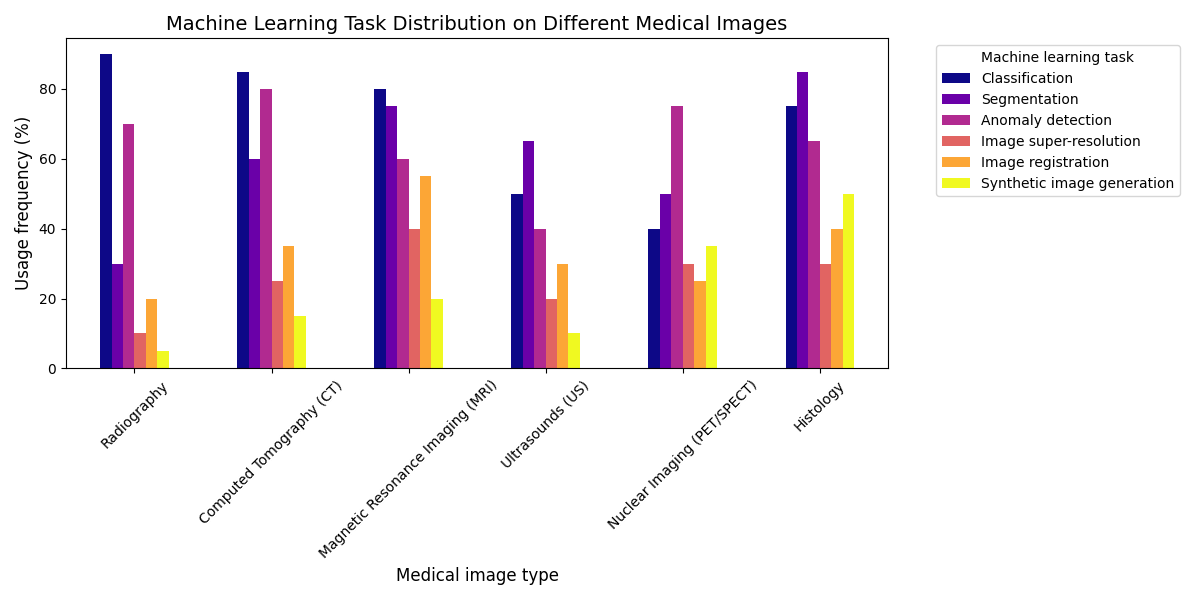
\includegraphics[width=0.9\textwidth]{Cap1/Figures/comparative-tasks-and-medical-image-types.png}
  \caption{Estimation of the popularity of tasks and medical image
    types based on
  recent literature review (count of referenced terms).}
  \label{fig:medical_image_analysis}
\end{figure}

For solving the different requirements of tasks in medical images, a
variety of computational techniques have been developed
\cite{Zhou2021}. Initially, these needs were covered with simple
morphological filters, which implied no training process or
elaborated optimization. However, as the complexity of the tasks
increased, the need for more sophisticated techniques arose, leading
to the application of advanced statistical tools and machine learning
algorithms like Support Vector Machines, Decision Trees, and SGD
Neural Networks \cite{Avanzo2024}. The coevolution of advances in medical image
acquisition, computational power (i.e. Moore's law) and
statistical/mathematical techniques have led to a convergence for
merging state of the art algorithms with medical imaging
\cite{Shalf2020}. Figure \ref{fig:medical-ai-timeline} shows a brief
timeline of coevolution between some conspicuous advances in
computational pattern recognition and its medical applications in
different scopes (besides medical imaging) \cite{Avanzo2024}.

\begin{figure}
  \centering
  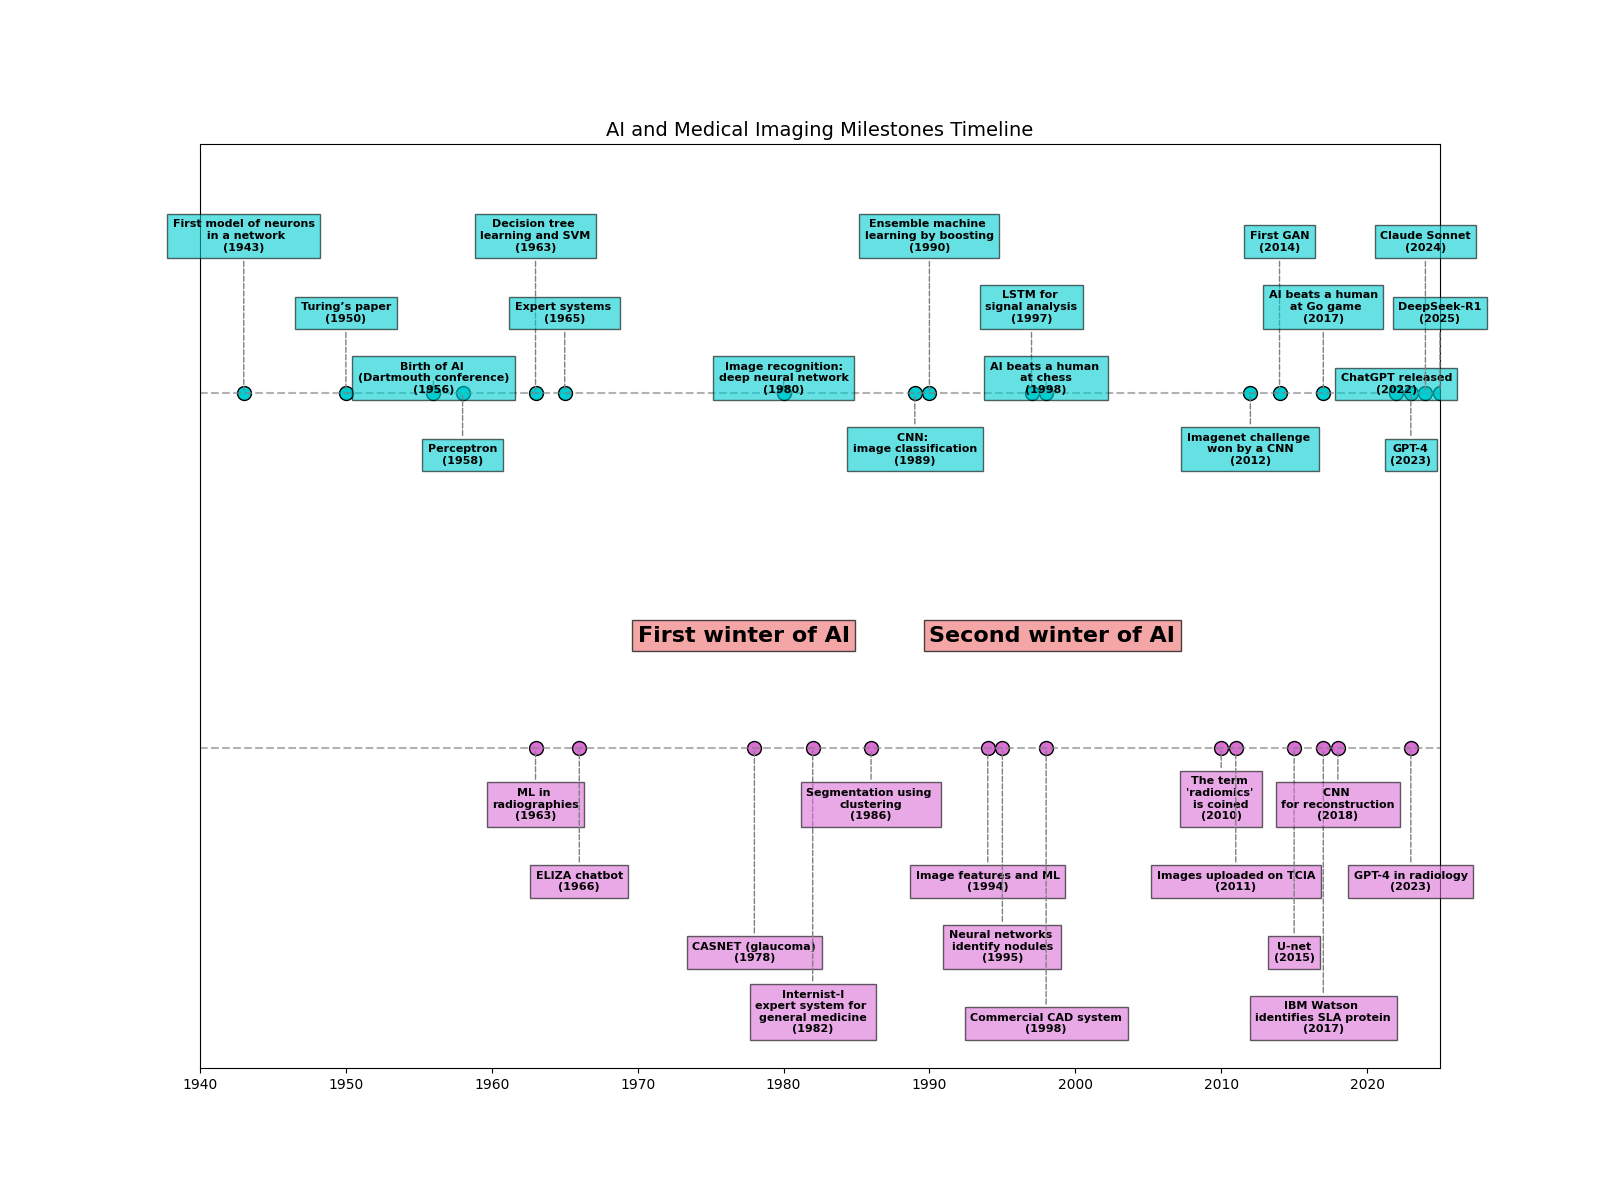
\includegraphics[trim={5cm 2cm 5cm
  0},width=0.9\textwidth]{Cap1/Figures/medical-ai-timeline.png}
  \caption{AI and machine learning in medical imaging brief timeline.}
  \label{fig:medical-ai-timeline}
\end{figure}

\gls{CNN} have been widely used in \gls{SS} tasks, as they have outperformed
traditional machine learning algorithms in this task for both medical
and non medical images \cite{XuYan2024} \cite{Sarvamangala2022}.
However, most \gls{CNN} architectures are deep, which imply
a necessity of a large amount of data to train them. This introduces
a problem since both the acquisition and annotation of medical images
are expensive and time-consuming processes. This is especially true
for \gls{ISS} tasks, as they require pixel-level annotations, which
is taxing in terms of cost, time and logistics involved
\cite{Bhalgat2018}. Other fashions face this problem through less expensive
annotation strategies like bounding boxes or anatomical landmarks for
being used in a semi-supervised strategy \cite{Shah2018}.

%% CHECKED

Many medical images datasets however, contain a high variability in
class sizes and variations in colors, which is specially noticeable
in histopathological images because of the usage of different
staining and other factors which can affect the color of the images
(see section \ref{sec:staining-techniques}).
This variability can lead to a significant loss of efficiency of
machine learning models when using a mixed supervision strategy, as
the model can be biased towards the most common classes or colors in
the dataset \cite{Shah2018}.

This is were other solutions arise to tackle the problem of the weak
image annotation while maintaining low costs. One of these solutions
is crowdsourcing strategy, which consists of having multiple annotators
labeling the same image, and then combining the labels to obtain a
consensus label \cite{LuEtAl2023}. This strategy can lead to a
labeling cost reduction when different levels of expertise are
combined, since the crowd may be composed of both experts and laymen,
being the latter less expensive to hire \cite{Lopez2023}.

Recently, diagnosis, prognosis and treatment of cancer have heavily
relied on histopathology, where tissue samples are obtained through biopsies or
surgical resections and critical information that helps
pathologists determine the presence and severity of malignancies
\cite{LopezEtAl2024}. The segmentation of histopathological images
enables precise identification of structures such as nuclei, glands, and tumors,
which are essential for assessing disease progression and treatment
response \cite{Rashmi2021}. Accurate segmentation is particularly
crucial in digital pathology, where whole-slide images (\gls{WSI})
are analyzed using AI-powered \gls{CAD} systems to support
clinical decision-making \cite{LopezEtAl2024}.

A major challenge in histopathological image segmentation arises from
the variability in annotations provided by different pathologists.
Unlike natural images, where object boundaries are often
well-defined, histological structures may have ambiguous borders,
leading to inconsistencies among annotators \cite{Lopez2023}. Because of this,
crowdsourcing labeling is one of the most popular approaches, as
illustrated in Figure \ref{fig:multiannotator_segmentation},
an example of how histopathological images are segmented by
multiple experts, showing some variations in label assignment
\footnote{obtained from a real world Triple Negative Breast
Cancer (TNBC) dataset published in \cite{Lopez2023}}. These
discrepancies highlight the need for models that can handle
annotation uncertainty effectively. Leveraging crowdsourcing
strategies and machine learning techniques that infer annotator
reliability can enhance segmentation performance while reducing costs.
\begin{figure}
  \centering
  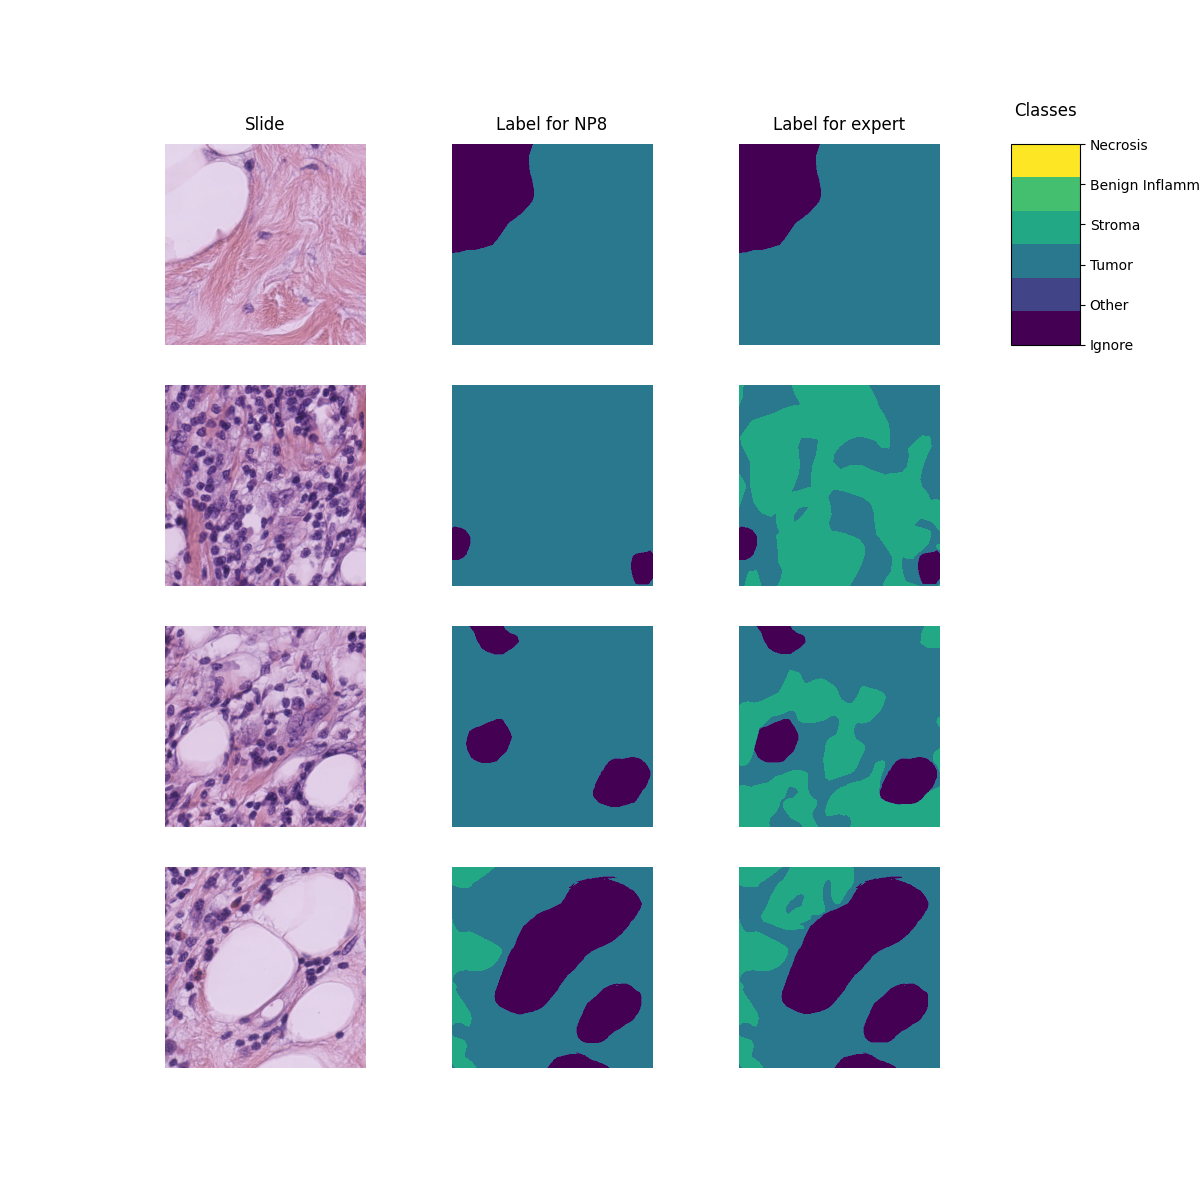
\includegraphics[width=0.9\textwidth]{Cap1/Figures/multiannotator-segmentation.png}
  \caption{Example of a histopathological image segmented by multiple
  annotators, illustrating variations in label assignment.}
  \label{fig:multiannotator_segmentation}
\end{figure}